%%%%%%%%%%%%%%%%%%%%%%%%%%%%%%%%%%%%%%%%%%%%%%%%%%%%%%%%%%%%%%%%%%%%%%%%%%%%
% AGUJournalTemplate.tex: this template file is for articles formatted with LaTeX
%
% This file includes commands and instructions
% given in the order necessary to produce a final output that will
% satisfy AGU requirements, including customized APA reference formatting.
%
% You may copy this file and give it your
% article name, and enter your text.
%
%
% Step 1: Set the \documentclass
%
%

%% To submit your paper:
\documentclass[draft]{agujournal2019}
\usepackage{url} 
\usepackage{graphicx,natbib,overpic,xcolor}
\usepackage{apacite}
%\bibliographystyle{unsrtnat}
%this package should fix any errors with URLs in refs.
\usepackage{lineno}
\usepackage[inline]{trackchanges} %for better track changes. finalnew option will compile document with changes incorporated.
\usepackage{soul}
\linenumbers
%%%%%%%
% As of 2018 we recommend use of the TrackChanges package to mark revisions.
% The trackchanges package adds five new LaTeX commands:
%
%  \note[editor]{The note}
%  \annote[editor]{Text to annotate}{The note}
%  \add[editor]{Text to add}
%  \remove[editor]{Text to remove}
%  \change[editor]{Text to remove}{Text to add}
%
% complete documentation is here: http://trackchanges.sourceforge.net/
%%%%%%%

\draftfalse

%% Enter journal name below.
%% Choose from this list of Journals:
%
% JGR: Atmospheres
% JGR: Biogeosciences
% JGR: Earth Surface
% JGR: Oceans
% JGR: Planets
% JGR: Solid Earth
% JGR: Space Physics
% Global Biogeochemical Cycles
% Geophysical Research Letters
% Paleoceanography and Paleoclimatology
% Radio Science
% Reviews of Geophysics
% Tectonics
% Space Weather
% Water Resources Research
% Geochemistry, Geophysics, Geosystems
% Journal of Advances in Modeling Earth Systems (JAMES)
% Earth's Future
% Earth and Space Science
% Geohealth
%
% ie, \journalname{Water Resources Research}

\journalname{Diurnal Aggregation}


\begin{document}

%% ------------------------------------------------------------------------ %%
%  Title
%
% (A title should be specific, informative, and brief. Use
% abbreviations only if they are defined in the abstract. Titles that
% start with general keywords then specific terms are optimized in
% searches)
%
%% ------------------------------------------------------------------------ %%

% Example: \title{This is a test title}

\title{Diurnal Self-Aggregation}

%% ------------------------------------------------------------------------ %%
%
%  AUTHORS AND AFFILIATIONS
%
%% ------------------------------------------------------------------------ %%

% Authors are individuals who have significantly contributed to the
% research and preparation of the article. Group authors are allowed, if
% each author in the group is separately identified in an appendix.)

% List authors by first name or initial followed by last name and
% separated by commas. Use \affil{} to number affiliations, and
% \thanks{} for author notes.
% Additional author notes should be indicated with \thanks{} (for
% example, for current addresses).

% Example: \authors{A. B. Author\affil{1}\thanks{Current address, Antartica}, B. C. Author\affil{2,3}, and D. E.
% Author\affil{3,4}\thanks{Also funded by Monsanto.}}

\authors{Jan O. Haerter}


% \affiliation{1}{First Affiliation}
% \affiliation{2}{Second Affiliation}
% \affiliation{3}{Third Affiliation}
% \affiliation{4}{Fourth Affiliation}

\affiliation{1}{Niels Bohr Institute, University of Copenhagen, Blegdamsvej 17, 2100 Copenhagen, Denmark}
%(repeat as many times as is necessary)

%% Corresponding Author:
% Corresponding author mailing address and e-mail address:

% (include name and email addresses of the corresponding author.  More
% than one corresponding author is allowed in this LaTeX file and for
% publication; but only one corresponding author is allowed in our
% editorial system.)

% Example: \correspondingauthor{First and Last Name}{email@address.edu}

\correspondingauthor{Jan O. Haerter}{haerter@nbi.ku.dk}

%% Keypoints, final entry on title page.

%  List up to three key points (at least one is required)
%  Key Points summarize the main points and conclusions of the article
%  Each must be 100 characters or less with no special characters or punctuation and must be complete sentences

% Example:
% \begin{keypoints}
% \item	List up to three key points (at least one is required)
% \item	Key Points summarize the main points and conclusions of the article
% \item	Each must be 100 characters or less with no special characters or punctuation and must be complete sentences
% \end{keypoints}

\begin{keypoints}
\item enter point 1 here
\item enter point 2 here
\item enter point 3 here
\end{keypoints}

%% ------------------------------------------------------------------------ %%
%
%  ABSTRACT and PLAIN LANGUAGE SUMMARY
%
% A good Abstract will begin with a short description of the problem
% being addressed, briefly describe the new data or analyses, then
% briefly states the main conclusion(s) and how they are supported and
% uncertainties.

% The Plain Language Summary should be written for a broad audience,
% including journalists and the science-interested public, that will not have 
% a background in your field.
%
% A Plain Language Summary is required in GRL, JGR: Planets, JGR: Biogeosciences,
% JGR: Oceans, G-Cubed, Reviews of Geophysics, and JAMES.
% see http://sharingscience.agu.org/creating-plain-language-summary/)
%
%% ------------------------------------------------------------------------ %%

%% \begin{abstract} starts the second page

\begin{abstract}
In contrast to the standard radiative convective equilibrium setup, where surface conditions are held constant, we make surface conditions diurnally oscillating.
While the atmosphere gradually equilibrates, and domain mean precipitation is similar from day to day, the spatial distribution of precipitation is only homogeneous during the first day. 
Already during the second day, the precipitation field is strongly structured and continues to cluster in subsequent days.
The clustering is robust to changes in resolution but can removed by reduction of the amplitude of oscillation.
Our results suggest that a modest diurnal cycle in forcing conditions can lead to aggregation-like structuring of the convective atmosphere. 
\end{abstract}

\section*{Plain Language Summary}
[ enter your Plain Language Summary here or delete this section]


%% ------------------------------------------------------------------------ %%
%
%  TEXT
%
%% ------------------------------------------------------------------------ %%

%%% Suggested section heads:
% \section{Introduction}
%
% The main text should start with an introduction. Except for short
% manuscripts (such as comments and replies), the text should be divided
% into sections, each with its own heading.

% Headings should be sentence fragments and do not begin with a
% lowercase letter or number. Examples of good headings are:

% \section{Materials and Methods}
% Here is text on Materials and Methods.
%
% \subsection{A descriptive heading about methods}
% More about Methods.
%
% \section{Data} (Or section title might be a descriptive heading about data)
%
% \section{Results} (Or section title might be a descriptive heading about the
% results)
%
% \section{Conclusions}


\section{Introduction}\label{sec:intro}
Convective self-aggregation is an idealized model for tropical convective precipitation over a sea surface of constant temperature.


\section{Methods}\label{sec:methods}
The convective atmosphere was simulated using the University of California, Los Angeles (UCLA) Large Eddy Simulation (LES) model with sub-grid scale turbulence parameterized after Smagorinsky \cite{smagorinsky}, a delta four-stream radiation scheme \cite{pincus} and a two-moment cloud microphysics scheme \cite{stevens2005evaluation}. 
Rain evaporation is implemented after \citeA{seifert2008parameterization}.
As detailed in \citeA{moseley2016intensification}, diurnally oscillating surface temperature ($T_s(t)$) boundary conditions are applied, with
\begin{eqnarray}
  T_s(t)=\overline{T_{s}}-T_{a} \cos{(t/t_0)}\;,
\end{eqnarray}
\noindent
with $\overline{T_{s}}=298\;K$ and $t_0=24;h$ is the duration of the simulated model day.
All simulations were initialized with data from observed summertime mid-latitude conditions where convection had occurred in order to establish an initially unstable atmosphere. 
However, due to the repeated diurnal cycle forcing, the system eventually establishes a self-consistent vertical temperature and moisture profile [show this somewhere].

\noindent
The model numerically integrates the anelastic equations of motion on a regular horizontal domain with varying horizontal grid spacing $dx$ and periodic boundary conditions. 
The model spans 75 stretchable vertical levels peaking at the full domain height of 16.5 km with a sponge layer above 12.3 km.
The Coriolis force and the mean wind were set to zero with weak random initial perturbations added as noise to break complete spatial symmetry. 
No large scale forcing was imposed,
ensuring that the only driving force for convection was buoyancy and the forced lifting through cold pool interaction.
The model output time step is $\Delta t_{out}=5\;min$. 
At each output time step, $5\;min$-accumulated precipitation and instantaneous velocities are output at each model gridbox. 

We carry out three distinct simulations:
\begin{itemize}
    \item {\bf A}: $T_a=5\;K$ and $dx=1\;km$,
    \item {\bf B}: $T_a=2\;K$ and $dx=1\;km$,
    \item {\bf C}: $T_a=5\;K$ and $dx=.5\;km$.
\end{itemize}


\section{Results}\label{sec:results}


\begin{figure*}
\centering
%\begin{overpic}
%\includegraphics[height=0.33\linewidth]{cavities}
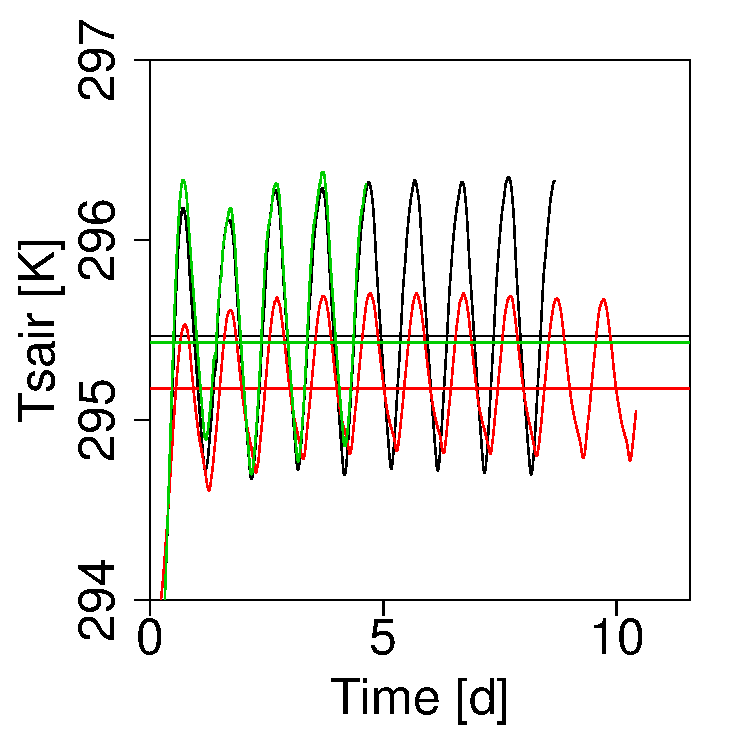
\includegraphics[trim={0 0 0cm 0}, clip, height=0.32\linewidth]{tsair_timeseries.pdf}
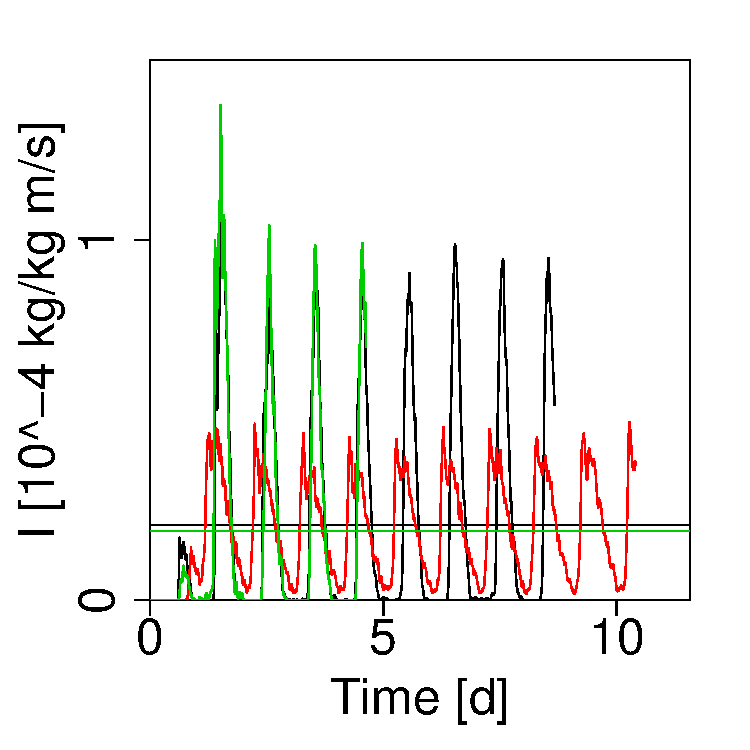
\includegraphics[trim={0 0 0cm 0}, clip, height=0.32\linewidth]{prcp_timeseries.pdf}
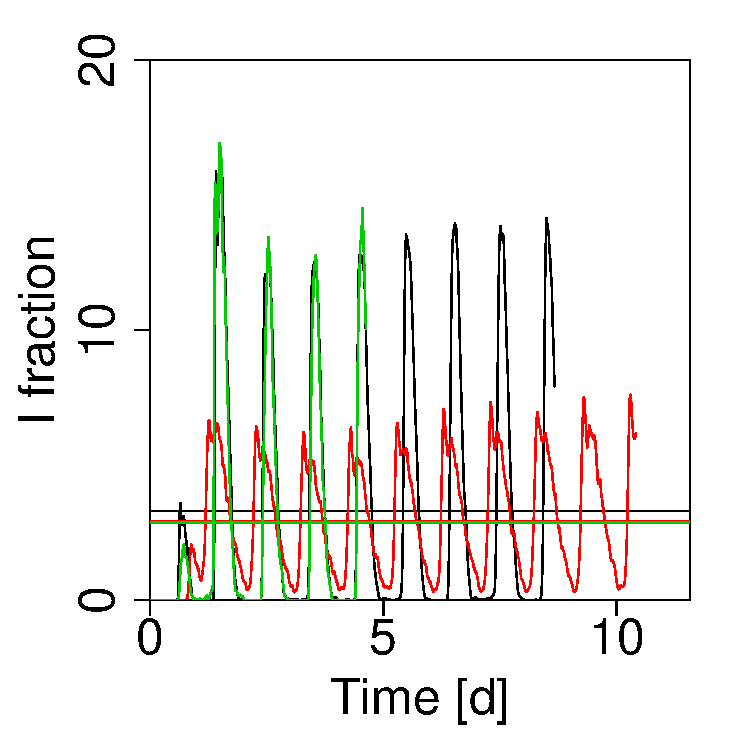
\includegraphics[trim={0 0 0cm 0}, clip, height=0.32\linewidth]{pfrac_timeseries.pdf}
\caption{{\bf Time series of domain averaged quantities}. }
\label{fig:domain_mean_timeseries}
\end{figure*}

\begin{figure*}
\centering
%\begin{overpic}
%\includegraphics[height=0.33\linewidth]{cavities}
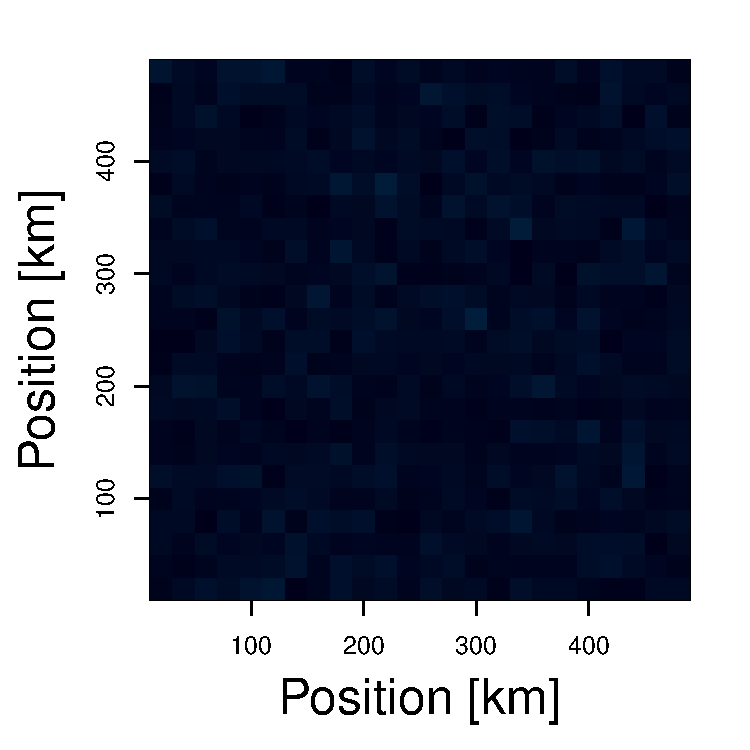
\includegraphics[trim={2cm 2cm 1cm 1cm}, clip, height=0.24\linewidth]{1-288_T0_300K_ampl_10_1km_r_int_timmean_xy_plot.pdf}
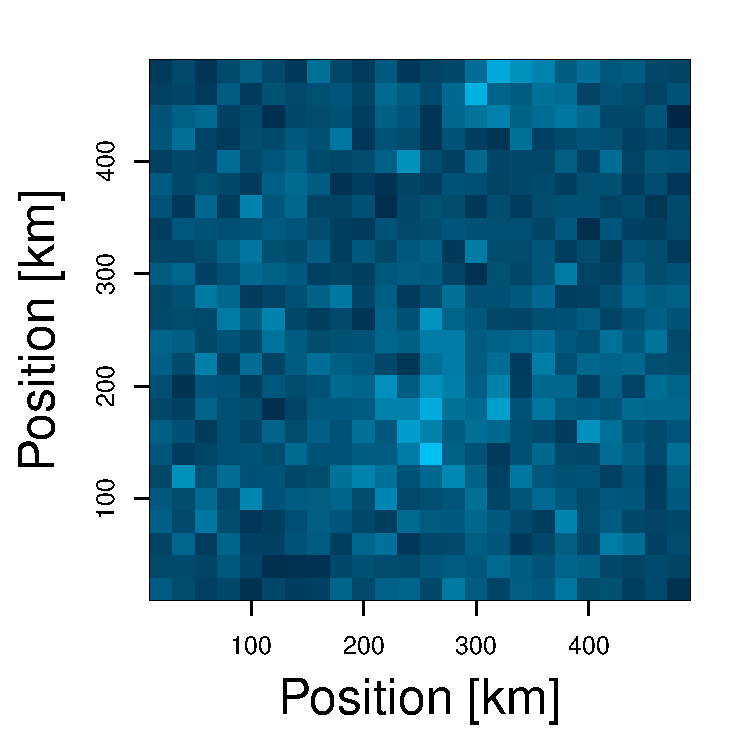
\includegraphics[trim={2cm 2cm 1cm 1cm}, clip, height=0.24\linewidth]{333-600_T0_300K_ampl_10_1km_r_int_timmean_xy_plot.pdf}
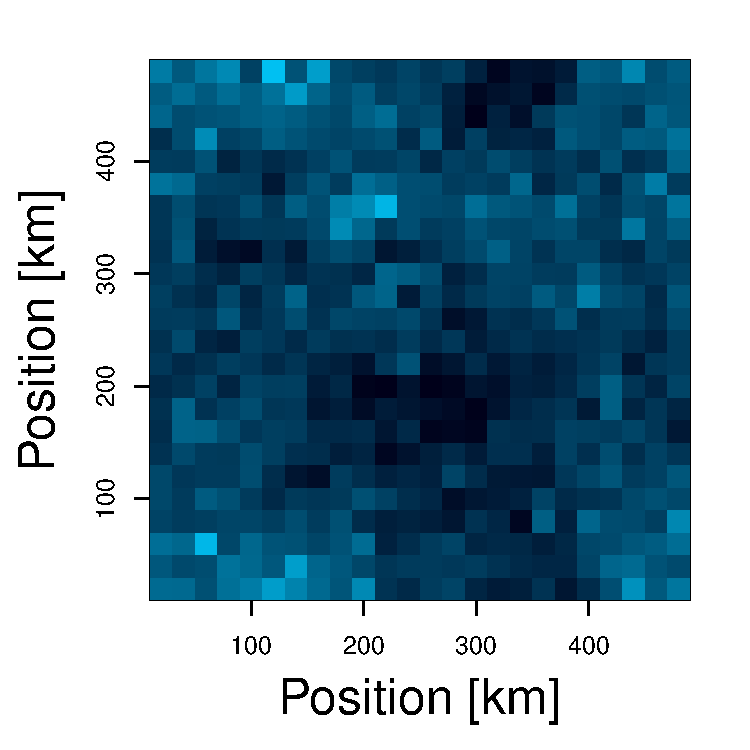
\includegraphics[trim={2cm 2cm 1cm 1cm}, clip, height=0.24\linewidth]{621-888_T0_300K_ampl_10_1km_r_int_timmean_xy_plot.pdf}
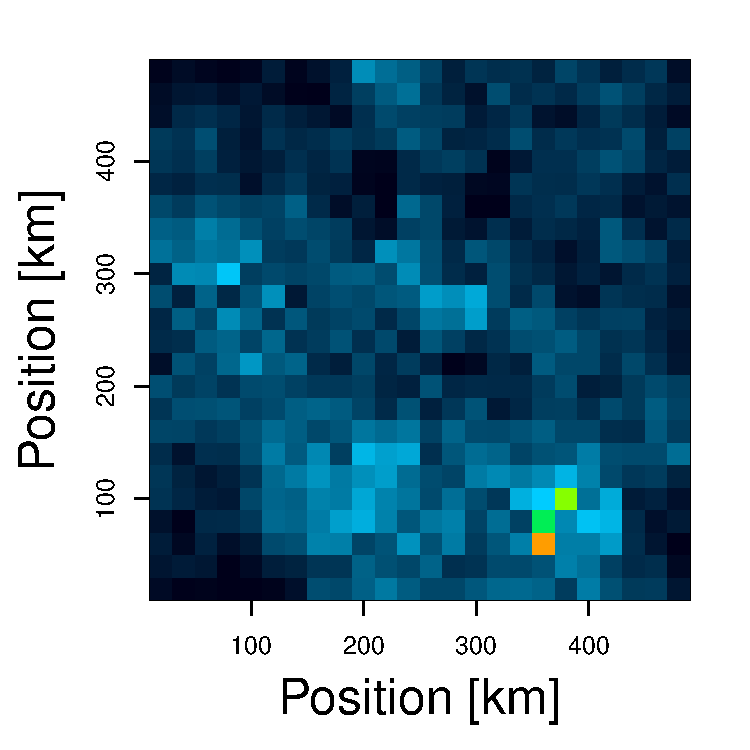
\includegraphics[trim={2cm 2cm 1cm 1cm}, clip, height=0.24\linewidth]{909-1176_T0_300K_ampl_10_1km_r_int_timmean_xy_plot.pdf}
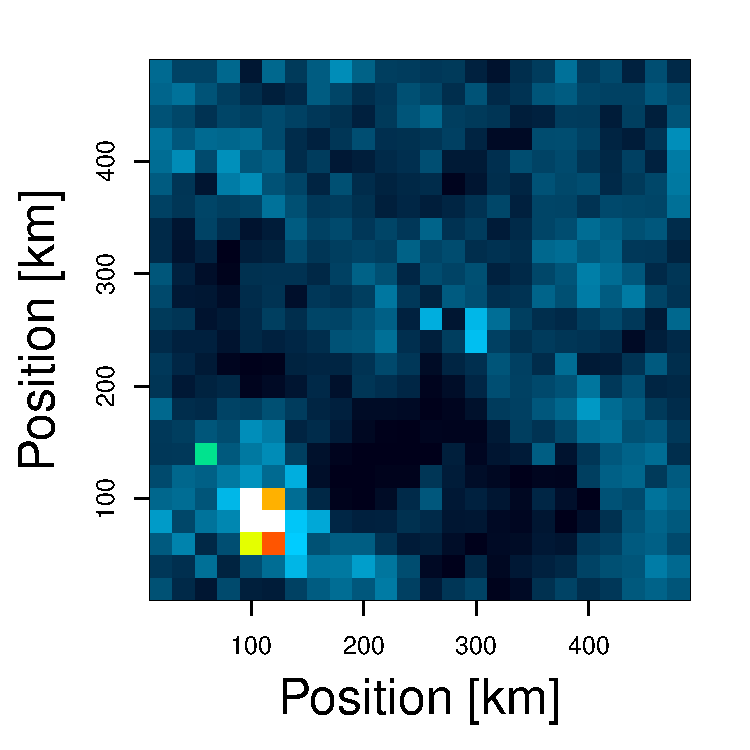
\includegraphics[trim={2cm 2cm 1cm 1cm}, clip, height=0.24\linewidth]{1197-1464_T0_300K_ampl_10_1km_r_int_timmean_xy_plot.pdf}
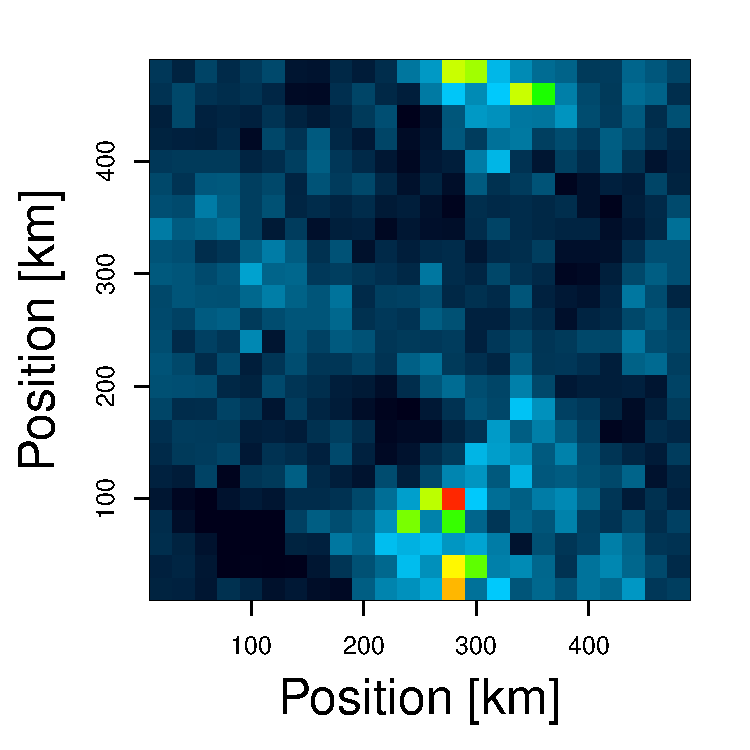
\includegraphics[trim={2cm 2cm 1cm 1cm}, clip, height=0.24\linewidth]{1485-1752_T0_300K_ampl_10_1km_r_int_timmean_xy_plot.pdf}
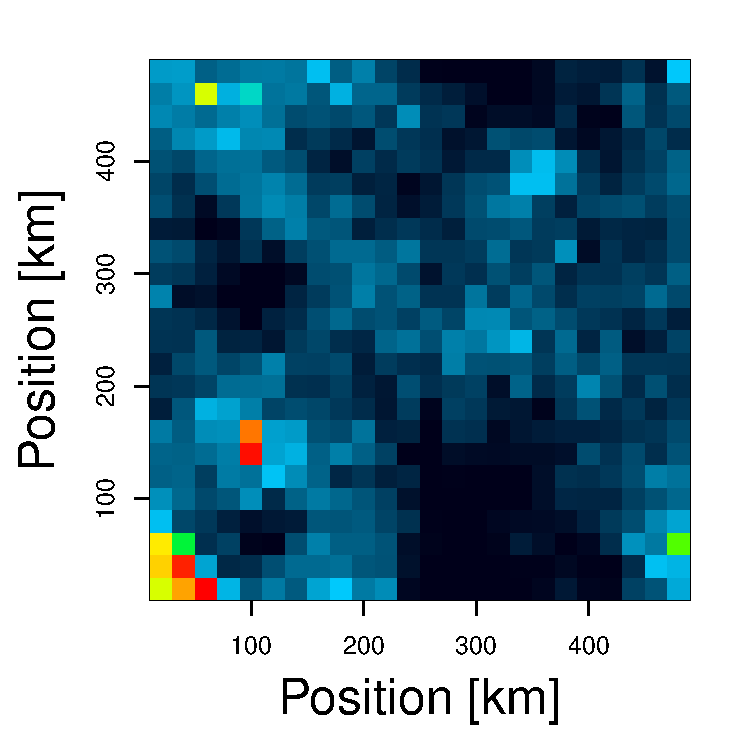
\includegraphics[trim={2cm 2cm 1cm 1cm}, clip, height=0.24\linewidth]{1773-2040_T0_300K_ampl_10_1km_r_int_timmean_xy_plot.pdf}
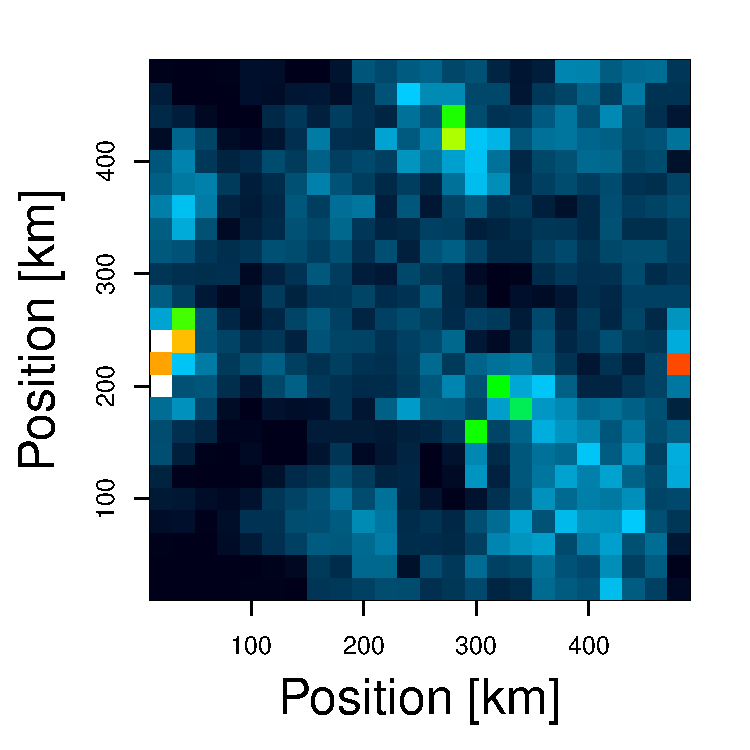
\includegraphics[trim={2cm 2cm 1cm 1cm}, clip, height=0.24\linewidth]{2061-2348_T0_300K_ampl_10_1km_r_int_timmean_xy_plot.pdf}
\caption{{\bf Spatial distribution of daily precipitation sum.}. }
\label{fig:daily_sum_5K}
\end{figure*}

\begin{figure*}
\centering
%\begin{overpic}
%\includegraphics[height=0.33\linewidth]{cavities}
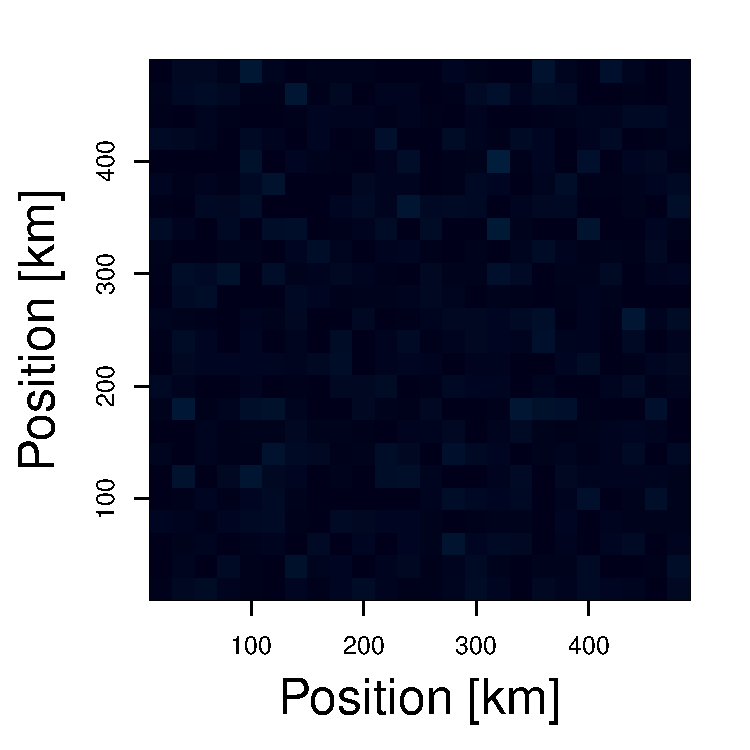
\includegraphics[trim={2cm 2cm 1cm 1cm}, clip, height=0.24\linewidth]{1-288_T0_300K_ampl_4_1km_r_int_timmean_xy_plot.pdf}
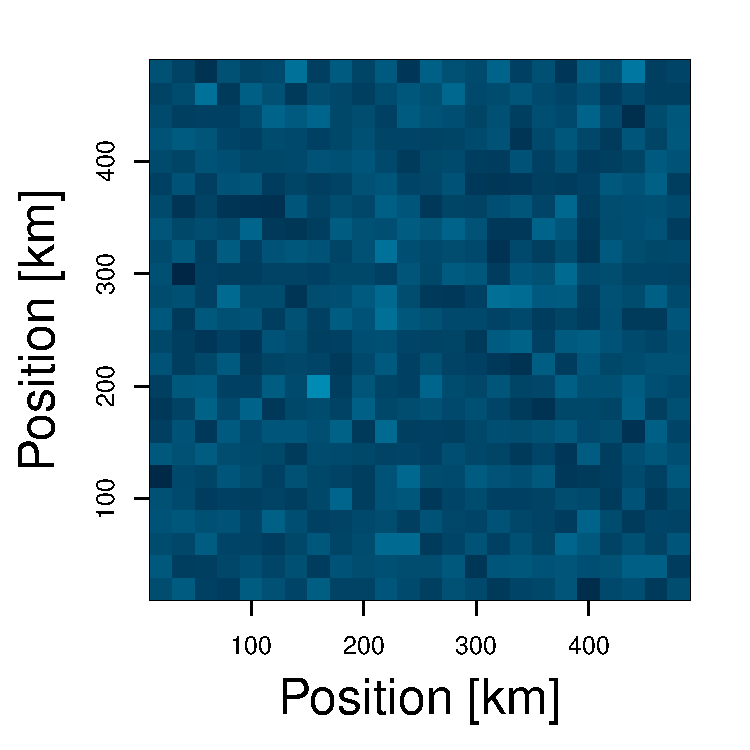
\includegraphics[trim={2cm 2cm 1cm 1cm}, clip, height=0.24\linewidth]{289-576_T0_300K_ampl_4_1km_r_int_timmean_xy_plot.pdf}
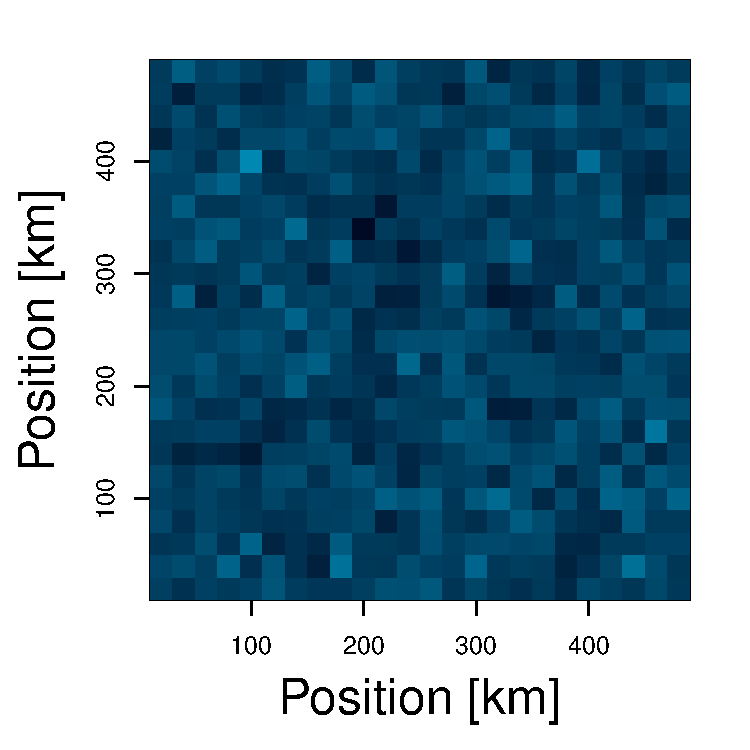
\includegraphics[trim={2cm 2cm 1cm 1cm}, clip, height=0.24\linewidth]{577-864_T0_300K_ampl_4_1km_r_int_timmean_xy_plot.pdf}
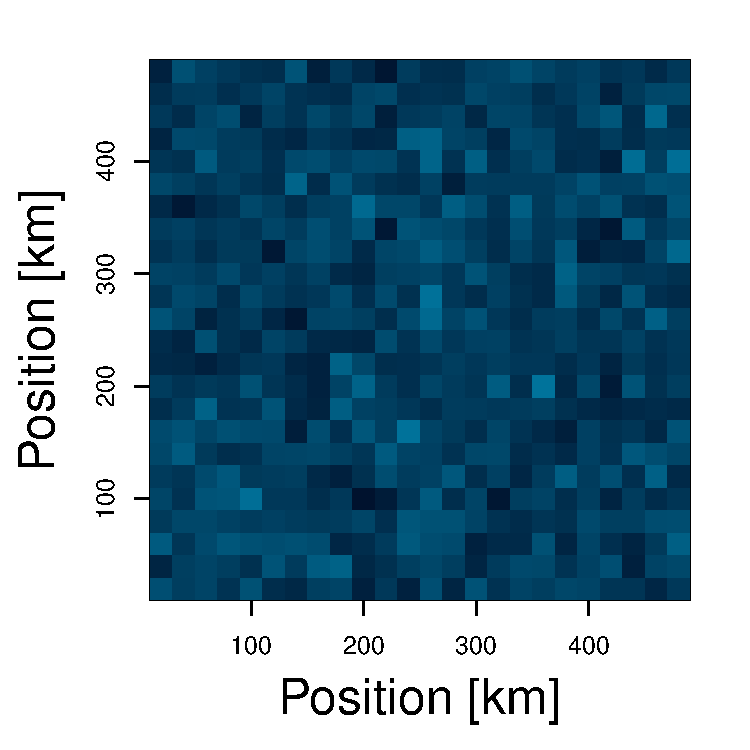
\includegraphics[trim={2cm 2cm 1cm 1cm}, clip, height=0.24\linewidth]{865-1172_T0_300K_ampl_4_1km_r_int_timmean_xy_plot.pdf}
\caption{{\bf Daily precipitation sum for smaller forcing amplitude.}. }
\label{fig:daily_sum_2K}
\end{figure*}


\begin{figure*}
\centering
%\begin{overpic}
%\includegraphics[height=0.33\linewidth]{cavities}
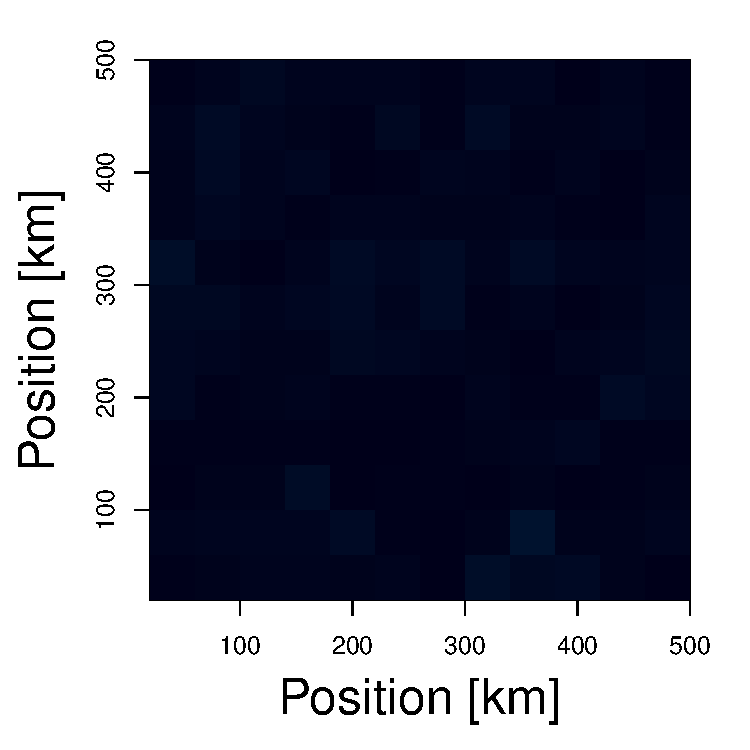
\includegraphics[trim={2cm 2cm 1cm 1cm}, clip, height=0.12\linewidth]{1-288_T0_300K_ampl_10_500m_r_int_timmean_xy_plot.pdf}
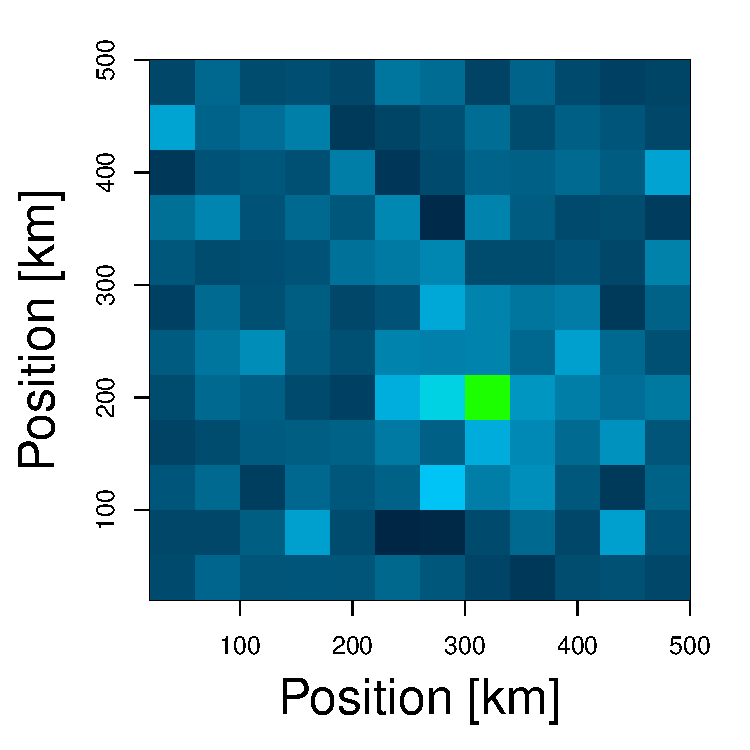
\includegraphics[trim={2cm 2cm 1cm 1cm}, clip, height=0.12\linewidth]{289-576_T0_300K_ampl_10_500m_r_int_timmean_xy_plot.pdf}
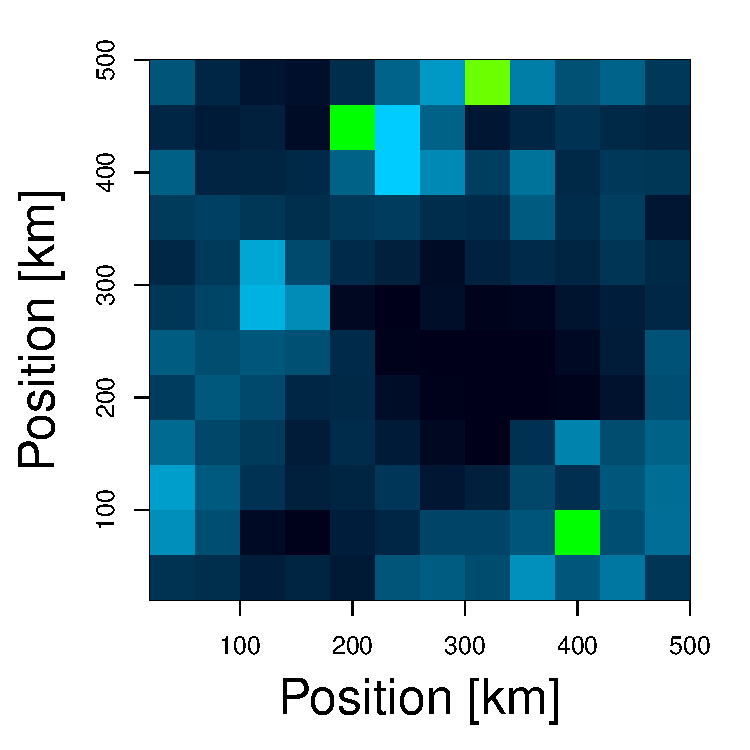
\includegraphics[trim={2cm 2cm 1cm 1cm}, clip, height=0.12\linewidth]{577-864_T0_300K_ampl_10_500m_r_int_timmean_xy_plot.pdf}
\caption{{\bf Daily precipitation sum for smaller forcing amplitude.}. }
\label{fig:daily_sum_2K}
\end{figure*}

\section{Discussion}\label{sec:discussions}

\section{Conclusion}\label{sec:conclusion}


\acknowledgments
JOH gratefully acknowledges funding by a grant from the VILLUM Foundation (grant number: 13168) and the European Research Council (ERC) under the European Union's Horizon 2020 research and innovation program (grant number: 771859).
The authors are grateful for computing resources and technical assistance provided by the Danish Center for Climate Computing, a facility built with support of the Danish e-Infrastructure Corporation, Danish Hydrocarbon Research and Technology Centre, VILLUM Foundation, and the Niels Bohr Institute.

\bibliography{references_clustering.bib}



%Reference citation instructions and examples:
%
% Please use ONLY \cite and \citeA for reference citations.
% \cite for parenthetical references
% ...as shown in recent studies (Simpson et al., 2019)
% \citeA for in-text citations
% ...Simpson et al. (2019) have shown...
%
%
%...as shown by \citeA{jskilby}.
%...as shown by \citeA{lewin76}, \citeA{carson86}, \citeA{bartoldy02}, and \citeA{rinaldi03}.
%...has been shown \cite{jskilbye}.
%...has been shown \cite{lewin76,carson86,bartoldy02,rinaldi03}.
%... \cite <i.e.>[]{lewin76,carson86,bartoldy02,rinaldi03}.
%...has been shown by \cite <e.g.,>[and others]{lewin76}.
%
% apacite uses < > for prenotes and [ ] for postnotes
% DO NOT use other cite commands (e.g., \citet, \citep, \citeyear, \nocite, \citealp, etc.).
%



\end{document}

